\section{LFSR as PRNG} \label{LFSR}
In this section we explain how CC2538 uses the CRC16 LFSR as a PRNG. 

\begin{figure}[!t]
\centering
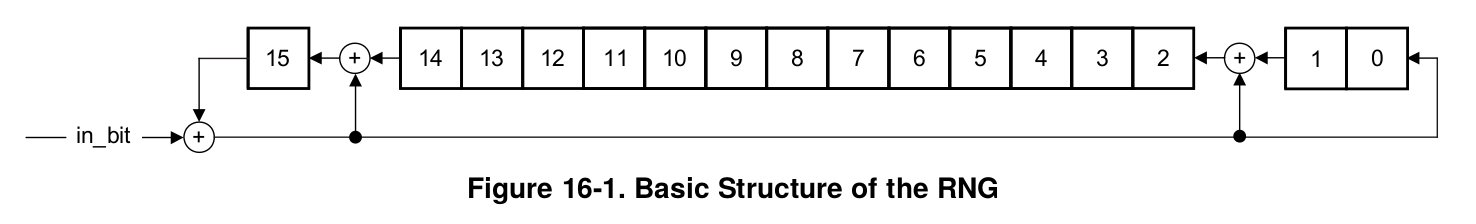
\includegraphics[width=2.5in]{fig/crc16.png}
\caption{CRC16 LFSR, from CC2538 User's Guide}
\label{CRC16}
\end{figure}

CC2538 User's Guide describes the PRNG design as: (Section 16.1 in CC2538 User's Guide)
\begin{quote}
The random-number generator is a 16-bit linear-feedback shift register (LFSR) with polynomial X 16 + X 15 +
X 2 + 1 (that is, CRC16). It uses different levels of unrolling depending on the operation it performs. The basic version (no unrolling) is shown in Figure 16-1 (\Cref{CRC16} in this paper).
\end{quote}

When used as a PRNG, the in\_bit of \Cref{CRC16} is constantly $0$. The Contiki driver calls the PRNG by: (Section 16.2.1in CC2538 User's Guide)
\begin{quote}
Another way to update the LFSR is to set the RCTRL bits in the SOC\_ADC\_ADCCON1 register to 01. This clocks the LFSR once (13x unrolling), and the RCTRL bits in the SOC\_ADC\_ADCCON1 register automatically clear when the operation completes.
\end{quote}

In another word, the LFSR is updated by performing 13 CRC16 operations in \Cref{CRC16}.

By nature, the LFSR based PRNG is stateful. Further more, the CRC16 operation is deterministic. Sine there are only 16 bits in the LFSR, we can denote the universal set of its  possible values $\mathbb{S}$ as:
\begin{equation} \label{PRNGState}
\mathbb{S} = \{ S_{i} | S_{i} \in \{2\}^{16}\}
\end{equation}
\Cref{PRNGState} also implies that the LFSR can have no more than $2^{16} = 65536$ values.

We also denote the LFSR update operation as:
\begin{equation}
F:\mathbb{S} \rightarrow \mathbb{S}
\end{equation}
where $F$ is the deterministic CRC16 operation.

Denote the random seed sampled by the radio noise as $S^*$. The PRNG can be formalised as:
\begin{equation}
	\begin{aligned}
	S_{0} &= S^* \\
	S_{i+1} &= F(S_{i})
	\end{aligned}
\end{equation}

Since ${S}$ is a finite set and $F$ is deterministic, the random number sequence $R$ generated by this PRNG can be represented as:
\begin{equation}
R= <F^0(S^{*}), >
\end{equation}

\section{Broken DTLS}
In this section we explain how to exploit the PRNG flaw to break ECDHE-ECDSA in DTLS handshake protocol.

\section{Reflection}
In this section we propose some idea to implement proper PRNGs on IoT devices.